\documentclass[12pt]{article}
\usepackage{amssymb,amsthm,amsmath}
\usepackage{mathtools}
\usepackage{lscape}

\usepackage{bigstrut}
%\usepackage{MnSymbol}
\usepackage{bbm}
\usepackage{proof}
\usepackage{bussproofs}
\usepackage{tikz}
\usepackage{lingmacros}
\usepackage{microtype}

\usepackage{setspace}
\usepackage{float}

\usepackage{tikz}
\usetikzlibrary{positioning,calc,arrows.meta,shapes.geometric,fit}

\usepackage{hyperref}
\definecolor{myblue}{rgb}{0.03, 0.27, 0.65}
\hypersetup{
    colorlinks,
    citecolor=myblue,
    filecolor=myblue,
    linkcolor=myblue,
    urlcolor=myblue
}

\usepackage{paralist}
\usepackage{enumitem}
\usepackage{etoolbox}
\AtBeginEnvironment{quote}{\par\singlespacing\small}

% Helpful spacing command
\newcommand{\compactcenter}[1]{\setlength{\abovedisplayskip}{0pt}{\[ #1 \]}}

\newcommand{\existsgeq}{\mbox{\sf AtLeast}}
\newcommand{\Pol}{\mbox{\emph{Pol}}}
  \newcommand{\nonered}{\textcolor{red}{=}}
  \newcommand{\equalsred}{\nonered}
  \newcommand{\redstar}{\textcolor{red}{\star}}
    \newcommand{\dred}{\textcolor{red}{d}}
    \newcommand{\dmark}{\dred}
    \newcommand{\redflip}{\textcolor{red}{flip}}
        \newcommand{\flipdred}{\textcolor{red}{\mbox{\scriptsize \em flip}\ d}}
        \newcommand{\mdred}{\textcolor{blue}{m}\textcolor{red}{d}}
        \newcommand{\ndred}{\textcolor{blue}{n}\textcolor{red}{d}}
\newcommand{\arrowm}{\overset{\textcolor{blue}{m}}{\rightarrow} }
\newcommand{\arrown}{\overset{\textcolor{blue}{n}}{\rightarrow} }
\newcommand{\arrowmn}{\overset{\textcolor{blue}{mn}}{\longrightarrow} }
\newcommand{\arrowmonemtwo}{\overset{\textcolor{blue}{m_1 m_2}}{\longrightarrow} }
\newcommand{\bluen}{\textcolor{blue}{n}}
\newcommand{\bluem}{\textcolor{blue}{m}}
\newcommand{\bluemone}{\textcolor{blue}{m_1}}
\newcommand{\bluemtwo}{\textcolor{blue}{m_2}}
\newcommand{\blueminus}{\textcolor{blue}{-}}

\newcommand{\bluedot}{\textcolor{blue}{\cdot}}
\newcommand{\bluepm}{\textcolor{blue}{\pm}}
\newcommand{\blueplus}{\textcolor{blue}{+ }}
\newcommand{\translate}[1]{{#1}^{tr}}
\newcommand{\Caba}{\mbox{\sf Caba}} 
\newcommand{\Set}{\mbox{\sf Set}} 
\newcommand{\Pre}{\mbox{\sf Pre}} 
\newcommand{\wmarkpolarity}{\scriptsize{\mbox{\sf W}}}
\newcommand{\wmarkmarking}{\scriptsize{\mbox{\sf Mon}}}
\newcommand{\smark}{\scriptsize{\mbox{\sf S}}}
\newcommand{\bmark}{\scriptsize{\mbox{\sf B}}}
\newcommand{\mmark}{\scriptsize{\mbox{\sf M}}}
\newcommand{\jmark}{\scriptsize{\mbox{\sf J}}}
\newcommand{\kmark}{\scriptsize{\mbox{\sf K}}}
\newcommand{\tmark}{\scriptsize{\mbox{\sf T}}}
\newcommand{\greatermark}{\mbox{\tiny $>$}}
\newcommand{\lessermark}{\mbox{\tiny $<$}}
%%{\mbox{\ensuremath{>}}}
\newcommand{\true}{\top}
\newcommand{\false}{\bot}
\newcommand{\upred}{\textcolor{red}{\uparrow}}
\newcommand{\downred}{\textcolor{red}{\downarrow}}
\usepackage[all,cmtip]{xy}
\usepackage{enumitem}
\usepackage{fullpage}
\usepackage[authoryear]{natbib}
\usepackage{multicol}
\theoremstyle{definition}
\newtheorem{definition}{Definition}
\newtheorem{theorem}{Theorem}
\newtheorem{lemma}[theorem]{Lemma}
\newtheorem{claim}{Claim}
\newtheorem{corollary}{Corollary}
%\newtheorem{theorem}{Theorem}
\newtheorem{proposition}{Proposition}
\newtheorem{example}{Example}
\newtheorem{remark}[theorem]{Remark}
\newcommand{\semantics}[1]{[\![\mbox{\em $ #1 $\/}]\!]}
\newcommand{\abovearrow}[1]{\rightarrow\hspace{-.14in}\raiseonebox{1.0ex}
{$\scriptscriptstyle{#1}$}\hspace{.13in}}
\newcommand{\toplus}{\abovearrow{r}}
\newcommand{\tominus}{\abovearrow{i}} 
\newcommand{\todestroy}{\abovearrow{d}}
\newcommand{\tom}{\abovearrow{m}}
\newcommand{\tomprime}{\abovearrow{m'}}
\newcommand{\A}{\textsf{App}}
\newcommand{\At}{\textsf{At}}
\newcommand{\Emb}{\textsf{Emb}}
\newcommand{\EE}{\mathbb{E}}
\newcommand{\DD}{\mathbb{D}}
\newcommand{\PP}{\mathbb{P}}
\newcommand{\QQ}{\mathbb{Q}}
\newcommand{\LL}{\mathbb{L}}
\newcommand{\MM}{\mathbb{M}}
\usepackage{verbatim}
\newcommand{\TT}{\mathcal{T}}
\newcommand{\Marking}{\mbox{Mar}}
\newcommand{\Markings}{\Marking}
\newcommand{\Mar}{\Marking}
\newcommand{\Model}{\mathcal{M}}
\newcommand{\Nodel}{\mathcal{N}}
\renewcommand{\SS}{\mathcal{S}}
\newcommand{\TTM}{\TT_{\Markings}}
\newcommand{\CC}{\mathbb{C}}
\newcommand{\erase}{\mbox{\textsf{erase}}}
\newcommand{\set}[1]{\{ #1 \}}
\newcommand{\arrowplus}{\overset{\blueplus}{\rightarrow} }
\newcommand{\arrowminus}{\overset{\blueminus}{\rightarrow} }
\newcommand{\arrowdot}{\overset{\bluedot}{\rightarrow} }
\newcommand{\arrowboth}{\overset{\bluepm}{\rightarrow} }
\newcommand{\arrowpm}{\arrowboth}
\newcommand{\arrowplusminus}{\arrowboth}
\newcommand{\arrowmone}{\overset{m_1}{\rightarrow} }
\newcommand{\arrowmtwo}{\overset{m_2}{\rightarrow} }
\newcommand{\arrowmthree}{\overset{m_3}{\rightarrow} }
\newcommand{\arrowmcomplex}{\overset{m_1 \orr m_2}{\longrightarrow} }
\newcommand{\arrowmproduct}{\overset{m_1 \cdot m_2}{\longrightarrow} }
\newcommand{\proves}{\vdash}
\newcommand{\Dual}{\mbox{\sc dual}}
\newcommand{\orr}{\vee}
\newcommand{\uar}{\uparrow}
\newcommand{\dar}{\downarrow}
\newcommand{\andd}{\wedge}
\newcommand{\bigandd}{\bigwedge}
\newcommand{\arrowmprime}{\overset{m'}{\rightarrow} }
\newcommand{\quadiff}{\quad \mbox{ iff } \quad}
\newcommand{\Con}{\mbox{\sf Con}}
\newcommand{\type}{\mbox{\sf type}}
\newcommand{\lang}{\mathcal{L}}
\newcommand{\necc}{\Box}
\newcommand{\vocab}{\mathcal{V}}
\newcommand{\wocab}{\mathcal{W}}
\newcommand{\Types}{\mathcal{T}_\mathcal{M}}
\newcommand{\mon}{\mbox{\sf mon}}
\newcommand{\anti}{\mbox{\sf anti}}
\newcommand{\FF}{\mathcal{F}}
\newcommand{\rem}[1]{\relax}


\newcommand{\raiseone}{\mbox{raise}^1}
\newcommand{\raisetwo}{\mbox{raise}^2}
\newcommand{\wrapper}[1]{{#1}}
\newcommand{\sfa}{\wrapper{\mbox{\sf a}}}
\newcommand{\sfb}{\wrapper{\mbox{\sf b}}}
\newcommand{\sfv}{\wrapper{\mbox{\sf v}}}
\newcommand{\sfw}{\wrapper{\mbox{\sf w}}}
\newcommand{\sfx}{\wrapper{\mbox{\sf x}}}
\newcommand{\sfy}{\wrapper{\mbox{\sf y}}}
\newcommand{\sfz}{\wrapper{\mbox{\sf z}}}
  \newcommand{\sff}{\wrapper{\mbox{\sf f}}}
    \newcommand{\sft}{\wrapper{\mbox{\sf t}}}
      \newcommand{\sfc}{\wrapper{\mbox{\sf c}}}
      \newcommand{\sfu}{\wrapper{\mbox{\sf u}}}
            \newcommand{\sfs}{\wrapper{\mbox{\sf s}}}
  \newcommand{\sfg}{\wrapper{\mbox{\sf g}}}

\newcommand{\sfvomits}{\wrapper{\mbox{\sf vomits}}}
\newlength{\mathfrwidth}
  \setlength{\mathfrwidth}{\textwidth}
  \addtolength{\mathfrwidth}{-2\fboxrule}
  \addtolength{\mathfrwidth}{-2\fboxsep}
\newsavebox{\mathfrbox}
\newenvironment{mathframe}
    {\begin{lrbox}{\mathfrbox}\begin{minipage}{\mathfrwidth}\begin{center}}
    {\end{center}\end{minipage}\end{lrbox}\noindent\fbox{\usebox{\mathfrbox}}}
    \newenvironment{mathframenocenter}
    {\begin{lrbox}{\mathfrbox}\begin{minipage}{\mathfrwidth}}
    {\end{minipage}\end{lrbox}\noindent\fbox{\usebox{\mathfrbox}}} 
 \renewcommand{\hat}{\widehat}
 \newcommand{\nott}{\neg}
  \newcommand{\preorderO}{\mathbb{O}}
 \newcommand{\PreorderP}{\mathbb{P}}
  \newcommand{\preorderE}{\mathbb{E}}
\newcommand{\preorderP}{\mathbb{P}}
\newcommand{\preorderN}{\mathbb{N}}
\newcommand{\preorderQ}{\mathbb{Q}}
\newcommand{\preorderX}{\mathbb{X}}
\newcommand{\preorderA}{\mathbb{A}}
\newcommand{\preorderR}{\mathbb{R}}
\newcommand{\preorderOm}{\mathbb{O}^{\bluem}}
\newcommand{\preorderPm}{\mathbb{P}^{\bluem}}
\newcommand{\preorderQm}{\mathbb{Q}^{\bluem}}
\newcommand{\preorderOn}{\mathbb{O}^{\bluen}}
\newcommand{\preorderPn}{\mathbb{P}^{\bluen}}
\newcommand{\preorderQn}{\mathbb{Q}^{\bluen}}
 \newcommand{\PreorderPop}{\mathbb{P}^{\blueminus}}
  \newcommand{\preorderEop}{\mathbb{E}^{\blueminus}}
\newcommand{\preorderPop}{\mathbb{P}^{\blueminus}}
\newcommand{\preorderNop}{\mathbb{N}^{\blueminus}}
\newcommand{\preorderQop}{\mathbb{Q}^{\blueminus}}
\newcommand{\preorderXop}{\mathbb{X}^{\blueminus}}
\newcommand{\preorderAop}{\mathbb{A}^{\blueminus}}
\newcommand{\preorderRop}{\mathbb{R}^{\blueminus}}
 \newcommand{\PreorderPflat}{\mathbb{P}^{\flat}}
  \newcommand{\preorderEflat}{\mathbb{E}^{\flat}}
\newcommand{\preorderPflat}{\mathbb{P}^{\flat}}
\newcommand{\preorderNflat}{\mathbb{N}^{\flat}}
\newcommand{\preorderQflat}{\mathbb{Q}^{\flat}}
\newcommand{\preorderXflat}{\mathbb{X}^{\flat}}
\newcommand{\preorderAflat}{\mathbb{A}^{\flat}}
\newcommand{\preorderRflat}{\mathbb{R}^{\flat}}
\newcommand{\pstar}{\preorderBool^{\preorderBool^{E}}}
\newcommand{\pstarplus}{(\pstar)^{\blueplus}}
\newcommand{\pstarminus}{(\pstar)^{\blueminus}}
\newcommand{\pstarm}{(\pstar)^{\bluem}}
\newcommand{\Reals}{\preorderR}
\newcommand{\preorderS}{\mathbb{S}}
\newcommand{\preorderBool}{\mathbbm{2}}
 \renewcommand{\o}{\cdot}
 \newcommand{\NP}{\mbox{\sc np}}
 \newcommand{\NPplus}{\NP^{\blueplus}}
  \newcommand{\NPminus}{\NP^{\blueminus}}
   \newcommand{\NPplain}{\NP}
    \newcommand{\npplus}{np^{\blueplus}}
  \newcommand{\npminus}{np^{\blueminus}}
   \newcommand{\npplain}{np}
   \newcommand{\np}{np}
   \newcommand{\Term}{\mbox{\sc t}}
  \newcommand{\N}{\mbox{\sc n}}
   \newcommand{\X}{\mbox{\sc x}}
      \newcommand{\Y}{\mbox{\sc y}}
            \newcommand{\V}{\mbox{\sc v}}
    \newcommand{\Nbar}{\overline{\mbox{\sc n}}}
    \newcommand{\Pow}{\mathcal{P}}
    \newcommand{\powcontravariant}{\mathcal{Q}}
    \newcommand{\Id}{\mbox{Id}}
    \newcommand{\pow}{\Pow}
   \newcommand{\Sent}{\mbox{\sc s}}
   \newcommand{\lookright}{\slash}
   \newcommand{\lookleft}{\backslash}
   \newcommand{\dettype}{(e \to t)\arrowminus ((e\to t)\arrowplus t)}
\newcommand{\ntype}{e \to t}
\newcommand{\etttype}{(e\to t)\arrowplus t}
\newcommand{\nptype}{(e\to t)\arrowplus t}
\newcommand{\verbtype}{TV}
\newcommand{\who}{\infer{(\nptype)\arrowplus ((\ntype)\arrowplus (\ntype))}{\mbox{who}}}
\newcommand{\iverbtype}{IV}
\newcommand{\Nprop}{\N_{\mbox{prop}}}
\newcommand{\VP}{{\mbox{\sc vp}}}
\newcommand{\CN}{{\mbox{\sc cn}}}
\newcommand{\Vintrans}{\mbox{\sc iv}}
\newcommand{\Vtrans}{\mbox{\sc tv}}
\newcommand{\Num}{\mbox{\sc num}}
%\newcommand{\S}{\mathbb{A}}
\newcommand{\Det}{\mbox{\sc det}}
\newcommand{\preorderB}{\mathbb{B}}
\newcommand{\simA}{\sim_A}
\newcommand{\simB}{\sim_B}
\newcommand{\polarizedtype}{\mbox{\sf poltype}}


\newcommand{\Prop}{\textsf{Prop}}
\newcommand{\Update}{\textsf{Update}}
\newcommand{\Inc}{\textsf{Inc}}
\newcommand{\AllNets}{\mathsf{Net}}
\newcommand{\Net}{\mathcal{N}}

\newcommand{\axiom}{\textsc}

\newcommand*{\bigchi}{\mbox{\Large$\chi$}}% big chi

\begin{document}
\title{Notes}
\maketitle
\renewcommand*\contentsname{\textcolor{myblue}{Jump to Section}}
\setstretch{0}
\tableofcontents
\singlespacing

%%%%%%%%%%%%%%%%%%%%%%%%%%%%%%%%%%%%%%%%%%%%%%%%%%%%
\section{\textcolor{myblue}{Introduction (from FLAIRS 2022)}}

\begin{abstract}
\begin{quote}
We present the logic of Hebbian learning, a dynamic logic whose semantics are expressed in terms of a layered neural network learning via Hebb's associative learning rule.  Its language consists of modality $\Box \varphi$ (read ``the propagation of signal $\varphi$'') as well as dynamic modalities $[\varphi^+] \psi$ (read ``evaluate $\psi$ after performing Hebbian update on $\varphi$'').  We give axioms and inference rules that are sound with respect to the neural semantics; these axioms characterize Hebbian learning and its interaction with propagation.  The upshot is that this logic describes a neuro-symbolic agent that both learns from experience and also reasons about what it has learned.
\end{quote}
\end{abstract}

Artificial intelligence  has  long  been  marked  by  a  schism between two of its major paradigms: symbolic reasoning and connectionist learning.  Neural systems have had wild success with learning from unstructured data, whereas symbolic reasoners are notorious for their rigidity.  On the other hand, symbolic systems excel at sophisticated (static) reasoning tasks that neural systems cannot readily learn.  Symbolic modules also tend to have more explainable reasoning, thanks to their use of explicit inferences in an intuitive language.  Moreover, due to their connection with logic, it is straightforward to compare the relative power and complexity of different symbolic reasoners.

But as Valiant famously put it, intelligent cognitive agents must have \emph{both} ``the ability to learn from experience, and the ability to reason from what has been learned'' \cite{valiant2003three}.  \emph{Neuro-symbolic artificial intelligence} has emerged in the last few decades to meet this challenge --- a monumental effort to integrate neural and symbolic systems, while retaining the advantages of both (see \cite{bader2005dimensions} and \cite{sarker2021neuro}, two surveys that span the decades).  Despite the cornucopia of neuro-symbolic proposals, the field has not yet agreed on an interface between the two that satisfyingly preserves both flexible learning and expressive reasoning.

Following the path set out by \cite{balkenius1991nonmonotonic} and \cite{leitgeb2001nonmonotonic,leitgeb2003nonmonotonic}, we advance the following proposal for the neuro-symbolic interface.  Rather than viewing the neural and symbolic as two different systems to be combined, we view them as two ways of interpreting the same agent.  More precisely, we view the dynamics of neural networks as the semantics to a formal logic.  This will immediately give us a formal correspondence between the chosen neural network model and this logic.

Previous work, particularly \cite{leitgeb2001nonmonotonic}, has considered how forward propagation in feed-forward nets forms a sound and complete semantics for the (static) conditional logic \textbf{CL} (\emph{loop-cumulative}).  The novelty of our paper is that we extend this logic by viewing a simple learning policy --- Hebbian update (``neurons that fire together wire together'') --- as a dynamic modality.  By doing so, we demonstrate that the dynamics of Hebbian learning (in feed-forward nets) directly corresponds to a particular multimodal logic that we call \emph{the logic of Hebbian learning}.  This logic meets Valiant's challenge:  It characterizes a cognitive agent that can learn from experience and also reason about what it has learned.

Our main result is the soundness of axioms and inference rules that characterize Hebbian learning.  The most interesting axioms involve the interaction between Hebbian update and forward propagation.  We also offer intuitive readings for the two modalities in terms of \emph{preference change}.  And although we leave the question of completeness open, we close by considering the importance of completeness for logics of this kind.

%%%%%%%%%%%%%%%%%%%%%%%%%%%%%%%%%%%%%%%%%%%%%%%%%%%%
\section{\textcolor{myblue}{Related Work (from FLAIRS 2022)}}

\textbf{Logics with Neural Semantics.}
As mentioned above, this work builds on \cite{balkenius1991nonmonotonic}, \cite{leitgeb2001nonmonotonic,leitgeb2003nonmonotonic}, which formally characterize the dynamics of a variety of inhibitory neural networks as corresponding conditional logics.  Similarly, \cite{blutner2004nonmonotonic} demonstrates that the Hopfield networks correspond to the logic of what he calls ``weight-annotated Poole systems.''  But the idea that we can view neural networks as the semantics for symbolic reasoning dates back to \cite{mcculloch1943logical}.  To date, no such neural semantics has tackled the issue of learning --- doing this for Hebbian update is precisely the contribution of our paper.

\textbf{Neuro-Symbolic AI.}
Across the neuro-symbolic literature, an ubiquitous premise is that integration involves combining or composing otherwise distinct neural and symbolic modules.  In contrast, this paper presents the neural and symbolic as two perspectives we can have about the same agent.

To our knowledge, the combined work work of \cite{garcez2001symbolic} and \cite{garcez2008neural} is the only neuro-symbolic proposal (besides neural semantics, see above) that exhibits this intimate interface between the two.  The former gives a formally sound method for extracting nonmonotonic rules from a network and the latter gives a method for build neural network models from rules (in a variety of different logics).  When combined, we can freely translate between a neural network and its beliefs.  But once again, unlike our work this framework does not offer a logical account of the neural network's learning.

% SAVE FOR JOURNAL VERSION
%Consider Henry Kautz' recent taxonomy of neuro-symbolic systems \cite{kautz-2020future}: All five of his categories involve combining or composing otherwise distinct neural and symbolic modules.

\textbf{Logics for Learning.}
Two recent papers, \cite{baltag2019dynamic} and \cite{baltag2019right}, also present dynamic modal logics that characterize learning.  The former models an individual's learning in the limit, whereas the latter models supervised learning as a game played between student and teacher.  But it is unclear how learning policies expressed in these logics might relate to specific neural implementations of learning, such as Hebbian update and backpropagation. 

%%%%%%%%%%%%%%%%%%%%%%%%%%%%%%%%%%%%%%%%%%%%%%%%%%%%
\section{\textcolor{myblue}{Neural Network Models}}

A model of the logic of Hebbian learning is just a special type of artificial neural network that we call a \emph{binary feedforward neural network} (BFNN).

\begin{definition} A BFNN is a pointed directed graph ${\Net = \langle N, E, W, T, A, \eta \rangle}$, where
\begin{itemize}
    \item $N$ is a finite nonempty set (the set of neurons)
    \item $E \subseteq N \times N$ (the set of excitatory connections)
    \item $W : N \times N \to \mathbb{R}$ (the weight of a given connection)
    \item $T$ is a function which maps each $n \in N$ to 
    $T^{(n)} \in \mathbb{R}$ (the threshold for $n$)
    
    % FOR JOURNAL VERSION:  Try to generalize
    % these results to work, replacing T with a generic output function (like Leitgeb does):
    %\item $O$ is a function which maps each $n \in N$ to
    %$O^{(n)} : \mathbb{R} \to \mathbb{R}$ (the output function for $n$)
    
    \item $A$ is a function which maps each $n \in N$ to\\
    $A^{(n)} : \mathbb{R}^k \to \mathbb{R}$ (the activation function for $n$, where $k$ is the indegree of $n$)
    \item $\eta \in \mathbb{R}, \eta \geq 0$ (the learning rate)
\end{itemize}
Moreover, BFNNs are \emph{feed-forward} in the sense that they do not contain cycles of edges with all nonzero weights.  BFNNs are \emph{binary} in the sense that the \emph{output} $O^{(n)} : \mathbb{R} \to \set{0, 1}$ of a neuron $n$ is given by $O^{(n)}(x) = 1$ iff $x \geq T^{(n)}$.

We further require that activation functions $A^{(n)}$ are
\begin{itemize}
    \item \textbf{(Nondecreasing)} For all $\vec{x}, \vec{y} \in \mathbb{R}^k$,
    if $\vec{x} \leq \vec{y}$ then $A^{(n)}(\vec{x}) \leq A^{(n)}(\vec{y})$
    
    \item \textbf{(Subadditive)} For all $\vec{x}, \vec{y} \in \mathbb{R}^k$,
    $A^{(n)}(\vec{x} + \vec{y}) \leq A^{(n)}(\vec{x}) + A^{(n)}(\vec{y})$
\end{itemize}
\end{definition}

This class of activation functions includes in particular the rectified linear activation function (ReLU).

We write $W_{ij}$ to mean $W(i,j)$, for ${(i, j) \in E}$.  When $m_i$ is drawn from a sequence ${m_1, \ldots, m_k}$, we can write ${A^{(n)}(\smash{\overrightarrow{W}}(m_i, n))}$ as shorthand instead of the full expression\\ $A^{(n)}(W(m_1, n), \ldots, W(m_k, n))$.


%%%%%%%%%%%%%%%%%%%%%%%%%%%%%%%%%%%%%%%%%%%%%%%%%%%
\section{\textcolor{myblue}{The $\Prop$ Function}}
Of course, BFNNs are not merely static directed graphs, but are dynamic in nature.  When a BFNN receives a signal (which we model as the initial state), it propagates that signal forward until the state of the net stabilizes.  This stable state of the net is considered to contain the net's response (answer) to the given signal (question).  We model forward propagation as follows, drawing heavily from the approach proposed by \cite{leitgeb2001nonmonotonic,leitgeb2018neural}.\footnote{Note that \cite{leitgeb2001nonmonotonic,leitgeb2018neural} defines propagation for \emph{inhibition nets}, i.e. weightless binary feed-forward networks whose dynamics are determined by both excitatory and inhibitory connections.  But later in this same paper, Leitgeb proves that inhibition nets and binary feed-forward networks (BFNNs) are equivalent with respect to their propagation structure.  And so we import his ideas and results here.}  

We consider a neuron $n$ active if its activation $A^{(n)}$ exceeds its threshold $T^{(n)}$ (intuitively, if the neuron fires).  Since our BFNNs are binary, either a given neuron is active ($1$) or it is not ($0$).  So we can identify the state of $\Net$ with a set of neurons that are active.  For a given BFNN $\Net$, let
\[
    \Set = \set{S \mid S \subseteq N}
\]
be its set of states.

A state $S \in \Set$ can further activate more neurons when the outputs of neurons in $S$ cause these new neurons' activations to exceed their thresholds.  Eventually, the state of $\Net$ stablizes.  We call this final state of affairs $\Prop(S)$, the \emph{propagation} of $S$.

\begin{definition}
Let $\Prop : \Set \to \Set$ be defined recursively as follows:  $n \in \Prop(S)$ iff either
\begin{itemize}
    \item[] \textbf{(Base Case)} $n \in S$, or
    \item[] \textbf{(Constructor)} There exist $m_1, \ldots, m_k \in \Prop(S)$ where each $(m_i, n) \in E$ and
    \[
    A^{(n)}(\smash{\overrightarrow{W}}(m_i, n)) \geq T^{(n)}
    \]
\end{itemize}
\end{definition}

Alternatively, consider a finite automaton with state space $\Set$ and transition function $F_{S^\ast} : \Set \to \Set$ tracking the propagation of an initial state $S^\ast$ through $\Net$.  We can view $\Prop(S^\ast)$ as a fixed point of $F_{S^\ast}$ \cite{leitgeb2001nonmonotonic}.
% COMMENT FOR JOURNAL VERSION:
% Leitgeb claims that Prop(S*) is *the unique* fixed point.  I'd like to be able to say this, but I should prove it myself for BFNNs.

The key insight of \cite{leitgeb2001nonmonotonic} is that we can neatly characterize the algebraic structure of $\Prop$ as a closure operator.

\begin{theorem}
Let $\Net \in \AllNets$.  For all $S, S_1, S_2 \in \Set$, $\Prop$ satisfies
\begin{itemize}
    \item \textbf{(Inclusion)} $S \subseteq \Prop(S)$
    
    \item \textbf{(Idempotence)} $\Prop(S) = \Prop(\Prop(S))$
    
    \item \textbf{(Distributivity)} 
    $\Prop(S_1) \cup \Prop(S_2) \subseteq \Prop(S_1 \cup S_2)$
    
    
    \item \textbf{(Cumulative)} If ${S_1 \subseteq S_2 \subseteq \Prop(S_1)}$ then ${\Prop(S_1) = \Prop(S_2)}$
    
    \item \textbf{(Loop)} If ${S_1 \subseteq \Prop(S_0)}, \ldots, {S_n \subseteq \Prop(S_{n-1})}$ and ${S_0 \subseteq \Prop(S_n)}$,\\ then ${\Prop(S_i) = \Prop(S_j)}$ for all $i, j \in \set{0, \ldots, n}$
\end{itemize}
\end{theorem}

\begin{proposition}
Crucially, $\Prop$ is \emph{not} monotonic.  I.e. it is not the case that for all $S_1, S_2 \in \Set$, if $S_1 \subseteq S_2$, then $\Prop(S_1) \subseteq \Prop(S_2)$.
\end{proposition}
\begin{proof}
Consider a net with three nodes, $a, b, c$ with $(a, b), (b, c) \in E$ and $W_{ab} = 1, W_{bc} = -1$, and a threshold of $T = 1$.  Let $S_1 = \set{a}, S_2 = \set{a, b}$.  $S_1 \subseteq S_2$, but $\Prop(S_1) = \set{a, c} \not \subseteq \set{a, b} = \Prop(S_2)$ (The negative $(b,c)$ edge inhibits the signal). [Drawing a picture would help here]
\end{proof}

But in place of monotonicity, $\Prop$ is \emph{loop-cumulative} (in the terminology of \cite{kraus1990nonmonotonic}).

%%%%%%%%%%%%%%%%%%%%%%%%%%%%%%%%%%%%%%%%%%%%%%%%%%%%
\section{\textcolor{myblue}{The $\Inc$ Function}}

The plan from here is to extend this logic of propagation by providing an account of Hebbian learning.  Our goal is to cast Hebbian update as a dynamic modality, so that we can explore its interactions with $\Prop$ in symbolic language.  As with $\Prop$, we start by outlining the algebraic structure of Hebbian update.

Hebb's classic learning rule \cite{hebb-organization-of-behavior-1949} states that when two adjacent neurons are simultaneously and persistently active, the connection between them strengthens.  In contrast with, e.g. backpropagation, Hebbian learning is errorless and unsupervised.  Another key difference is that Hebbian update is local --- the change in a weight $\Delta W_{ij}$ depends only on the activation of the immediately adjacent neurons.  For this reason, the Hebbian family of learning policies has traditionally been considered more biologically plausible than backpropagation.  There are many variations of Hebbian learning, but we only consider the most basic (unstable) form of Hebb's rule:  $\Delta W_{ij} = \eta x_i x_j$, where $\eta$ is the learning rate and $x_i, x_j$ are the outputs of adjacent neurons $i$ and $j$, respectively.

In order to incorporate Hebb's rule into our framework, we introduce a function $\Inc$ (``increase the weights'') to strengthen those neurons in a BFNN $\Net$ that are active when we feed $\Net$ a signal (initial state) $S \in \Set$.  
% SAVE EXPOSITION FOR THE JOURNAL
% ALSO needs to be rephrased, technically incorrect
%We can get the output of a neuron $n$ via the following characteristic function.
\begin{definition}
For $S \in \Set$, let 
$\bigchi_S : N \to \set{0, 1}$ be given by $\bigchi_S(n) = 1$ iff $n \in S$
\end{definition}

% SAVE EXPOSITION FOR THE JOURNAL
% $\Inc$ can now be defined as follows.
\begin{definition}
Let $\Inc : \AllNets \times \Set \to \AllNets$ be such that $\Inc(\langle N, E, W, T, A, \eta \rangle, S) = \langle N, E, W^\ast, T, A, \eta \rangle$, where
\[
    W_{ij}^\ast = W_{ij} + \eta \cdot \bigchi_{\Prop(S)}(i) \cdot  \bigchi_{\Prop(S)}(j)
\]
\end{definition}
Notice that we propagate $S$ before getting the active status of neurons.  
This is because otherwise
%when a Hebbian net receives a signal $S$, it strengthens all connections that are activated by $S$.  
%Otherwise, 
we would never strengthen connections beyond the input layer.

We were able to formulate the algebraic properties of $\Prop$ in terms of $\Set$ containment.  Similarly, we express the properties of $\Inc$ in terms of $\AllNets$ containment.  
% SAVE EXPOSITION FOR JOURNAL VERSION
%We define the notion of \emph{subnet} ($\preceq$) as follows.

\begin{definition}
Let $\Net_1, \Net_2 \in \AllNets$ differ only in their weight and threshold functions.  We write
\[
    \Net_1 \preceq \Net_2
\]
to mean that for all $S \in \Set$, $\Prop_{\Net_1}(S) \subseteq \Prop_{\Net_2}(S)$.  We use $\cong$ in the usual way to express that $\Net_1 \preceq \Net_2$ and $\Net_2 \preceq \Net_1$.
\end{definition}

For example, $\Inc(\Net, S)$ is a supernet of $\Net$ because strengthening weights via the $\Inc$ operation only has the potential to \emph{expand} future propagations.  To further cement this intuition, consider the least upper bound $\mathcal{N}^{lub}$ of $\preceq$.  $\mathcal{N}^{lub}$ is that net whose weights have been ``maximally'' strengthened, and so every propagation $\Prop(S)$ results in the entire set $N$.

% SAVE EXPOSITION FOR JOURNAL
% The following lemma states that if we would like to check the  $\Prop_{\Net_1}(S) \subseteq \Prop_{\Net_2}(S)$ condition, we can instead compare the weights and thresholds between $\Net_1$ and $\Net_2$ for neurons within $\Prop_{\Net_1}(S)$.

We have the following test to determine if $\Net_1$ is a subnet of $\Net_2$.

\begin{lemma}
\label{lemma:subnet->leq}
Suppose $\Net_1$ and $\Net_2$ are the same except for their weight and threshold functions, and let $S \in \Set$.  Then $\Prop_{\Net_1}(S) \subseteq \Prop_{\Net_2}(S)$ iff for all $m_1, \ldots, m_k, n \in \Prop_{\Net_1}(S)$ with $(m_i, n) \in E$,
\begin{equation}\tag{$\ast$}
\label{eqn:weight-condition}
  \begin{gathered}
    A^{(n)}(\smash{\overrightarrow{W}}_{\Net_1}(m_i, n)) \geq T_{\Net_1}^{(n)} \\
    \mbox{implies} \\
    A^{(n)}(\smash{\overrightarrow{W}}_{\Net_2}(m_i, n)) \geq T_{\Net_2}^{(n)}
  \end{gathered}
\end{equation}
\end{lemma}
\begin{proof}
($\rightarrow$) Consider the contrapositive; suppose we have $m_1, \ldots, m_k, n \in \Prop_{\Net_1}(S)$ such that 
\[
A^{(n)}(\smash{\overrightarrow{W}}_{\Net_1}(m_i, n)) \geq T_{\Net_1}^{(n)}
\]
but
\[
A^{(n)}(\smash{\overrightarrow{W}}_{\Net_2}(m_i, n)) < T_{\Net_2}^{(n)}
\]
Let $S = \set{m_1, \ldots, m_k}$.  Then $n \in \Prop_{\Net_1}(S)$, but $n \not \in \Prop_{\Net_2}(S)$.  So $\Net_1 \not \preceq \Net_2$.


($\leftarrow$) We want to show that $\Prop_{\Net_1}(S) \subseteq \Prop_{\Net_2}(S)$.  I'll show this by structural induction on $\Prop_{\Net_1}(S)$:

\textbf{Base Step:} $\Prop_{\Net_1}(S) = S$.  But then if $n \in S$, $n \in \Prop_{\Net_2}(S)$ by the base case of $\Prop_{\Net_2}(S)$.

\textbf{Inductive Step:}
$n \in \Prop_{\Net_1}(S)$ because there exist $m_1, \ldots, m_k \in \Prop_{\Net_1}(S)$ such that for all $i$, $(m_i, n) \in E$ and
\[
A^{(n)}(\smash{\overrightarrow{W}}_{\Net_1}(m_i, n)) \geq T_{\Net_1}^{(n)}
\]
By assumption,
\[
A^{(n)}(\smash{\overrightarrow{W}}_{\Net_2}(m_i, n)) \geq T_{\Net_2}^{(n)}
\]
Since all $m_i \in \Prop_{\Net_1}(S)$, by IH all $m_i \in \Prop_{\Net_2}(S)$.  And so $n \in \Prop_{\Net_2}(S)$ (by definition).
\end{proof}

\begin{corollary}
\label{corollary:subnet->weights}
Let $\Net_1, \Net_2$ be the same except for their weight and threshold functions.  Then $\Net_1 \preceq \Net_2$ iff for all $m_1, \ldots, m_k, n \in N$, (\ref{eqn:weight-condition}) holds.
\end{corollary}
\begin{proof}
($\rightarrow$) Suppose $\Net_1 \preceq \Net_2$.  Then for all $S$, $\Prop_{\Net_1}(S) \subseteq \Prop_{\Net_2}(S)$.  In particular, this holds for $S = N$.  By Lemma~\ref{lemma:subnet->leq}, (\ref{eqn:weight-condition}) holds for $\Prop_{\Net_1}(N) = N$.

($\leftarrow$) Suppose for all $m_1, \ldots, m_k, n \in N$, (\ref{eqn:weight-condition}) holds.  Let $S \in \Set, n \in \Prop_{\Net_1}(S)$.  So there exist $m_1, \ldots, m_k$ satisfying the antecedent of (\ref{eqn:weight-condition}).  And so the consequent holds, i.e. $n \in \Prop_{\Net_2}(S)$.
\end{proof}

Notice that the right-hand side of this biconditional does not mention $\Prop$; this test reduces the \emph{dynamic} condition ($\Net_1 \preceq \Net_2$) to a \emph{static} condition (a statement about the relative weights and thresholds between $\Net_1$ and $\Net_2$).

%%%%%%%%%%%%%%%%%%%%%%%%%%%%%%%%%%%%%%%%%%%%%%%%%%%%%%
\section{\textcolor{myblue}{Properties of $\Inc$}}

We have the following following algebraic characterization of $\Inc$.

\begin{theorem}
For all $\Net, \Net_1, \Net_2 \in \AllNets$ and $S, S_1, S_2 \in \Set$, $\Inc$ satisfies
\begin{itemize}
    \item \textbf{(Inclusion)}
    $\Net \preceq \Inc(\Net, S)$
    
    \item \textbf{(Absorption)}
    $\Inc(\Net, \Prop(S)) \cong \Inc(\Net, S)$
    
    \item \textbf{(Monotonicity in $\Net$)} if ${\Net_1 \preceq \Net_2}$
    then ${\Inc(\Net_1, S) \preceq \Inc(\Net_2, S)}$
    
    \item \textbf{(Iteration)}
    $\Inc(\Net, S_1 \cup \Prop_{\Inc(\Net, S_1)}(S_2))
    \preceq \Inc(\Inc(\Net, S_1), S_2)$
    
    \item \textbf{(Distributivity)}
    $\Prop_{\Inc(\Net, S_1)}(S) \cup \Prop_{\Inc(\Net, S_2)}(S)
    \subseteq \Prop_{\Inc(\Net, S_1 \cup S_2)}(S)$
    
    \item \textbf{(Local)}
    $\Prop_{\Inc(\Net, S_2)}(S_1) \subseteq \Prop_\Net(S_1) \cup \Prop_\Net(S_2)$
    
    \item \textbf{(Cumulative)} If ${\Prop_\Net(S_1) \subseteq \Prop_\Net(S_2)} \subseteq \Prop_{\Inc(\Net, S)}(S_1)$,\\
    then $\Prop_{\Inc(\Net, S)}(S_1) = \Prop_{\Inc(\Net, S)}(S_2)$
    
    \item \textbf{(Loop)} If ${\Prop_\Net(S_1) \subseteq \Prop_{\Inc(\Net, S)}(S_0)}$,
    $\ldots, {\Prop_\Net(S_n) \subseteq \Prop_{\Inc(\Net, S)}(S_{n-1})}$,\\
    and 
    ${\Prop_\Net(S_0) \subseteq \Prop_{\Inc(\Net, S)}(S_n)}$,\\
    then ${\Prop_{\Inc(\Net, S)}(S_i) = \Prop_{\Inc(\Net, S)}(S_j)}$
    for all $i, j \in \set{0, \ldots, n}$
\end{itemize}
\end{theorem}
\begin{proof}:
\begin{compactitem}
    \item \textbf{(Inclusion)}  
    
    \item \textbf{(Absorption)} 
    
    \item \textbf{(Monotonicity in $\Net$)} 
    
    \item \textbf{(Iteration)}
    
    \item \textbf{(Distributivity)}
    
    \item \textbf{(Local)}
    
    \item \textbf{(Cumulative)} 
    
    \item \textbf{(Loop)} 
    
\end{compactitem}
\end{proof}


% SAVE FOR JOURNAL VERSION!
% (we don't have space to spare here)
\begin{figure}
\centering{
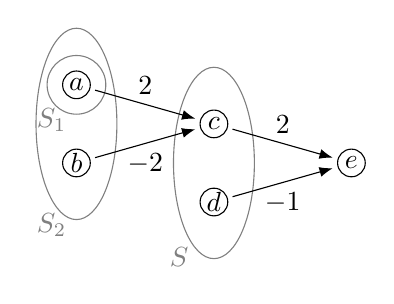
\begin{tikzpicture}[loose/.style={inner sep=.7em},edge/.style = {->,-Latex},
oval/.style={ellipse,draw}]

% nodes
\node[circle,minimum size=10pt,inner sep=0pt,outer sep=2pt,fill=white,draw](a){$a$};
\node[below=0.5 of a,circle,minimum size=10pt,inner sep=0pt,outer sep=2pt,fill=white,draw](b){$b$};

\node[right=1.5 of $(a)!0.5!(b)$,circle,minimum size=10pt,inner sep=0pt,outer sep=2pt,fill=white,draw](c){$c$};
\node[below=0.5 of c,circle,minimum size=10pt,inner sep=0pt,outer sep=2pt,fill=white,draw](d){$d$};

\node[right=1.5 of $(c)!0.5!(d)$,circle,minimum size=10pt,inner sep=0pt,outer sep=2pt,fill=white,draw](e){$e$};

% ovals
\node[oval,color=gray,fit=(a),inner sep=0.5pt]{};
\node[oval,color=gray,fit=(a) (b)]{};
\node[oval,color=gray,fit=(c) (d)]{};

% oval labels
\node [color=gray,left=0.005 of $(a)!0.45!(b)$]{$S_1$};
\node [color=gray,left=0.005 of $(a)!1.80!(b)$]{$S_2$};
\node [color=gray,left=0.2 of $(c)!1.70!(d)$]{$S$};

% edges
\draw[edge] (a) -- (c) node [midway, above] {$2$};
\draw[edge] (b) -- (c) node [midway, below] {$-2$};
\draw[edge] (c) -- (e) node [midway, above] {$2$};
\draw[edge] (d) -- (e) node [midway, below] {$-1$};
\end{tikzpicture}
}
\caption{todo}
\label{fig:monotonicity-counterexample}
\end{figure}


Like $\Prop$, $\Inc$ is loop-cumulative (in $S$).  But also like $\Prop$, $\Inc$ is not monotonic in $S$.  Consider a BFNN $\Net$ with ${N = \set{a, b, c, d, e}}$, ${W_{ab} = W_{ce} = 2}$, ${W_{bc} = -2}$, ${W_{de} = -1}$, and ${T = 2}$.
We have ${\Prop_{\Net_1}(S_1) = \set{a, c, e}}$, whereas $\Prop_{\Net_2}(S_2)$ = $\set{a, b}$ $= {S_2}$.  This means that $\Inc(\Net, S_1)$ increases the weights of ${a \to c}, {c \to e}$, while $\Inc(\Net, S_2)$ has no effect on the weights of $\Net$.  And so ${S_1 \subseteq S_2}$, yet $\Prop_{\Inc{\Net, S_1}}(S) = \set{c, d, e} \not \subseteq \set{c, d} = \Prop_{\Inc{\Net, S_2}}(S)$.

%%%%%%%%%%%%%%%%%%%%%%%%%%%%%%%%%%%%%%%%%%%%%%%%%%%%%%
\section{\textcolor{myblue}{Syntax and Semantics}}

We can now introduce the logic of Hebbian learning.  Let $p, q, \ldots$ be finitely many propositional variables.  These represent fixed, `ontic' states, i.e. established choices of neurons that correspond to features in the external world.  For example, $p$ might be the set of neurons that encapsulates the color \emph{pink}.  We presume that we already agree on these states, although we acknowledge that this is a major unresolved empirical issue.  As for more complex formulas:

\begin{definition}  The formulas of our language $\lang$ are given by
\[
\varphi \Coloneqq p \mid \top \mid \neg \varphi \mid \varphi \land \varphi \mid \varphi \to \varphi \mid \Box \varphi \mid [\varphi^+] \varphi
\]
where $p$ is any propositional variable.  We define $\bot, \lor, \leftrightarrow$ and the dual modalities $\Diamond, \langle \varphi^+ \rangle$ in the usual way.
\end{definition}

The modalities $\Box$ and $[\varphi^+]$ reflect our two operations $\Prop$ and $\Inc$, respectively.  We intend for $\Box \varphi$ to denote ``the propagation of signal $\varphi$,'' and for $[\varphi^+] \psi$ to denote ``after performing Hebbian update on $\varphi$, evaluate $\psi$.''  We will soon offer more classical, truth-conditional readings of $\Box$ and $[\varphi^+]$, but for now we content ourselves with these neural denotations.

A model of our logic is just a BFNN $\Net$ equipped with an interpretation function $\semantics{\cdot} : \lang \to \Set_\Net$. 
%(we write $\semantics{\cdot}$ when $\Net$ is unambiguous).

\begin{definition}
Let $\Net \in \AllNets$.  Our semantics are defined recursively as follows:
\begin{equation*}
\boxed{
\begin{array}{lcl}
\semantics{p} & & \in \Set \mbox{ is fixed, nonempty} \\
\semantics{\top} & = & \emptyset \\
\semantics{\neg \varphi} & = & \overline{\semantics{\varphi}}\\
\semantics{\varphi \land \psi} & = & \semantics{\varphi} \cup \semantics{\psi}\\
\semantics{\varphi \to \psi} & = & \semantics{\top} \textrm{ iff } \semantics{\varphi} \supseteq \semantics{\psi}\\
\semantics{\Box \varphi} & = & \Prop(\semantics{\varphi}) \\
\semantics{[\varphi^+] \psi} & = & \semantics{\psi}_{\Inc(\Net, \semantics{\varphi})} \\
\end{array}
}
\end{equation*}
\end{definition}

It may seem odd that we interpret $\land$ as union (instead of intersection), $\to$ as superset (instead of subset), and $\top$ as $\emptyset$ (instead of $N$).  But this choice reflects the intuition that neurons act as ``elementary-feature-detectors'' \cite{leitgeb2001nonmonotonic}.  For example, say $\semantics{\varphi}$ represents those neurons that detect whether an object is a car, and $\semantics{\psi}$ represents those neurons that detect the color yellow.  If the net observes a yellow car ($\varphi \land \psi$), \emph{both} sets of neurons $\semantics{\varphi}$ and $\semantics{\psi}$ activate.  As for $\to$, ``every car is yellow'' ($\varphi \to \psi$) means that whenever a car is detected, the color yellow must be detected as well.  That is, the set of neurons detecting car-features $\semantics{\varphi}$ must \emph{contain} those neurons detecting yellow-features $\semantics{\psi}$.  This justifies us reading propositional connectives classically, despite the backwards flavor of the semantics.

Note that Leitgeb's conditional $\varphi \Rightarrow \psi$ is equivalent to the formula $\Box \varphi \to \psi$ \cite{leitgeb2001nonmonotonic}.  With our earlier intuition that a propagation contains the answer to the given question, this crucial formula says that the net \emph{classifies} $\varphi$ as $\psi$.  The reason for our notational facelift is that $\Box$ is more fine-grained than $\Rightarrow$, which allows our language to capture certain subtle interactions between propagation and Hebbian update.

Our interpretation of formulas is completely algebraic, in the sense that formulas denote sets rather than truth-values.  But we can consider formulas to have truth-values as follows.

\begin{definition}
$\Net \models \varphi$ iff $\semantics{\varphi}_\Net = \emptyset$.
\end{definition}
\begin{figure}[ht!]
\begin{equation*}
\boxed{
\begin{array}{ll}
    & \textbf{Basic Axioms}\\
    
    \axiom{(PC)} & \mbox{All proposotional tautologies}\\

    \axiom{(Dual)} & \Diamond \varphi \leftrightarrow \neg \Box \neg \varphi\\
    
    \axiom{(M)} & \Box(\varphi \land \psi) \to (\Box \varphi \land \Box \psi)\\
    
    % \axiom{(M2)} & (\Box \varphi \orr \Box \psi) \to \Box(\varphi \orr \psi)\\
    
    \axiom{(N)} & \Box \top\\
    
    \axiom{(T)} & \Box \varphi \to \varphi\\
    
    \axiom{(4)} & \Box \varphi \to \Box \Box \varphi\\
    
    & \textbf{Inference Rules}\\

    \axiom{(MP)} & \frac{\varphi \quad \varphi \to \psi}{\psi} \\

    (\axiom{Nec}_\Box) & \frac{\varphi}{\Box \varphi} \\
    (
    \axiom{Nec}_+) & \frac{\psi}{[\varphi^+] \psi} \\
    
    (\axiom{C}_\Box) & \frac{\varphi \to \psi \quad \Box \psi \to \varphi}{\Box \varphi \leftrightarrow \Box \psi} \\
    
    (\axiom{C}_+) & \frac{\psi \to \rho \quad [\varphi^+] \rho \to \psi}{[\varphi^+] \psi \leftrightarrow [\varphi^+] \rho} \\
    
    (\axiom{Loop}_\Box) & 
    \frac{\Box \varphi_0 \to \varphi_1
    \cdots
    \Box \varphi_{k-1} \to \varphi_k \enskip
    \Box \varphi_k \to \varphi_0}
    {\Box \varphi_0 \to \varphi_k} \\
    
    (\axiom{Loop}_+) & \frac{[\varphi^+] \psi_0 \to \psi_1 
    \cdots 
    [\varphi^+] \psi_{k-1} \to \psi_k \enskip 
    [\varphi^+] \psi_k \to \psi_0}
    {[\varphi^+] \psi_0 \to \psi_k} \\
    
    & \textbf{Reduction Axioms}\\

    (\axiom{R}_p) & [\varphi^+] p \leftrightarrow p \\
    
    (\axiom{R}_\neg) & [\varphi^+] \neg \psi \leftrightarrow \neg [\varphi^+] \psi \\
    
    (\axiom{R}_\land) & [\varphi^+] (\psi \land \rho) \leftrightarrow ([\varphi^+] \psi \land [\varphi^+] \rho)\\
    
    & \textbf{Key Axioms}\\
    
    \axiom{(Iter)} & [\varphi^+] [\psi^+] \rho \to [(\varphi \land [\varphi^+] \psi)^+] \rho \quad\\
    
    % Reductions of neSted terms.
    % (\axiom{Nest}_\neg) & [\neg \varphi^+] \psi \leftrightarrow \psi \orr \neg [\varphi^+] \psi\\
    
    (\axiom{Nest}_\land) & [(\varphi \land \psi)^+] \rho \to ([\varphi^+] \rho \land [\psi^+] \rho)\\
    
    (\axiom{Nest}_\Box) & [\Box \varphi^+] \psi \leftrightarrow [\varphi^+] \psi \\

    % Agent prefers the result of update in advance
    % "No Disappointment"
    \axiom{(ND)} & [\varphi^+] \Box \psi \to \Box [\varphi^+] \psi\\
    
    % "Preference Persistence"
    % (one of the four major effects under the umbrella of "confirmation bias"
    \axiom{(PP)} & \Box [\varphi^+] \psi \land \Box \varphi \to [\varphi^+] \Box \psi\\
\end{array}
}
\end{equation*}
\caption{A list of sound rules and axioms of the logic of Hebbian learning.}
\label{fig:proof-system}
\end{figure}

This choice also appears to be strange at its surface.  But it is a natural one in light of the fact that we defined $\semantics{\top} \coloneqq \emptyset$.  For example, consider implication: $\Net \models \varphi \to \psi$ holds iff $\semantics{\varphi \to \psi} = \emptyset = \semantics{\top}$, which is exactly the condition $\semantics{\varphi} \supseteq \semantics{\psi}$ we gave for implication.

A curious consequence is that if $\Net \models \varphi$ and $\varphi$ cannot be written to contain an implication $\to$, then $\varphi$ must be a tautology.  But we do not consider this troubling, since it only makes sense to consider a neural network's judgment of $\varphi$ when given a state $\semantics{\psi}$ the net is in.

%%%%%%%%%%%%%%%%%%%%%%%%%%%%%%%%%%%%%%%%%%%%%%%%%%%%%%%%
\section{\textcolor{myblue}{Inference and Axioms}}

The proof system for our logic is the usual modal one: We have $\proves \varphi$ iff either $\varphi$ is an axiom, or $\varphi$ follows from previously obtained formulas by one of the inference rules.  If $\Gamma \subseteq \lang$ is a set of formulas, we consider $\Gamma \proves \varphi$ to hold whenever there exist finitely many $\psi_1, \ldots, \psi_k$ such that $\proves \psi_1 \land \ldots \land \psi_k \to \varphi$.

We list the axioms and inference rules for our logic in Figure~\ref{fig:proof-system}.  Our main result is the soundness of these axioms and rules --- we do not claim that this list forms a complete axiomatization (we revisit the question of completeness in the Conclusion).

The static base of our logic is formed by the non-normal modal logic \textbf{EMNT4}, along with inference rules $(\axiom{C}_\Box), (\axiom{Loop}_\Box)$ expressing the loop-cumulativity of $\Prop$.  This fragment of the proof system is just the conditional logic \textbf{CL} re-cast in terms of $\Box$.

Like $\Box$, we have the inference rules $(\axiom{Nec}_+)$, $(\axiom{C}_+)$, $(\axiom{Loop}_+)$ for $[\varphi^+]$ (the latter two express the loop-cumulativity of $\Inc$).  Since Hebbian update only affects the propagation of states, we have reduction axioms $(\axiom{R}_p), (\axiom{R}_\neg), (\axiom{R}_\land)$.  In lieu of a full reduction for $[\varphi^+] \Box \psi$, we instead have the weaker axioms $\axiom{(ND)}$ and $\axiom{(PP)}$.  Finally, we also have axioms that deal with nested terms $(\axiom{Nest}_\land) (\axiom{Nest}_\Box)$ and repeated iteration $(\axiom{Iter})$.

% COMMENT TO MAKE ON THE JOURNAL VERSION:
% Notes: we give reductions in terms of \neg and \land (which covers implication, top, and bot), primarily because of the lemma that makes nested implications useless (so we have to rephrase (K) for [\varphi^+], for instance)

% COMMENT TO MAKE ON THE JOURNAL VERSION:
% To check the validity of each of these axioms and rules, we make use of the following technical fact.  Notice that it follows that antecedents in right-associated implications get absorbed, e.g. $\varphi \to (\psi \to \rho)$ reduces to $\psi \to \rho$.
% \begin{lemma}
% Suppose $S \ne N$.  Then $\Net, S \models \varphi \to \psi$ iff $\Net, \semantics{\varphi}_\Net \models \psi$ (iff $\semantics{\psi}_\Net \subseteq \semantics{\varphi}_\Net$).
% \end{lemma}

%%%%%%%%%%%%%%%%%%%%%%%%%%%%%%%%%%%%%%%%%%%%%%%%%%%%%%%%
\section{\textcolor{myblue}{Soundness}}

Soundness of the above axioms is just a matter of matching each axiom with its corresponding property of $\Inc$.

\begin{theorem}
The rules and axioms above are sound, i.e. hold for all $\Net \in \AllNets$.
\end{theorem}
\begin{proof}

\end{proof}

%%%%%%%%%%%%%%%%%%%%%%%%%%%%%%%%%%%%%%%%%%%%%%%%%%%%%%%%
\section{\textcolor{myblue}{Completeness}}



%%%%%%%%%%%%%%%%%%%%%%%%%%%%%%%%%%%%%%%%%%%%%%%%%%%%%%%%
\section{\textcolor{myblue}{Reducibility}}



\section{\textcolor{myblue}{$[\varphi^+]$ as Preference Change}}

One of the key advantages of symbolic systems is their explainability.  Typically, symbolic languages have an intuitive reading that help explain their inferences.  But so far, we have not given a clear English reading of $\Box \varphi$ and $[\varphi^+] \psi$, divorced from the dynamics of neural networks.  Here we argue for an account of $\Box \varphi$ and $[\varphi^+] \psi$ in terms of \emph{preference change}.

%Recall that our $\Box$ is inter-translatable with the conditional $\varphi \Rightarrow \psi$ of \textbf{CL} via $\Box \varphi \to \psi$.  

In the literature on nonmonotonic reasoning, $\varphi \Rightarrow \psi$ is interpreted as ``typical $\varphi$ are $\psi$,'' where $\varphi$ and $\psi$ are read as generics (e.g. `cars' and `yellow things').  Since in our logic we can express this conditional as $\Box \varphi \to \psi$, it follows that $\Box \varphi$ by itself represents of the net's `typical $\varphi$.'\footnote{As further support for this typicality reading, note that our $\Box$ strongly resembles the typicality operator \textbf{T} introduced into the DL $\mathcal{ALC}$ by \cite{giordano2009alc+}.  Similar to our $\Box$, \textbf{T} is inter-translatable with conditionals $\varphi \Rightarrow \psi$ via \textbf{T}$(\varphi) \sqsubseteq \psi$ (notice the subtle flip in the direction of containment).}

% Since our $\Box$ is inter-translatable with the conditional $\varphi \Rightarrow \psi$ of \textbf{CL} (via $\Box \varphi \to \psi$), we are inclined to read
% \[
% \Net \models \Box \varphi
% \]
% as ``the net $\Net$ believes that $S$ is a typical $\varphi$.''

Philosophers use the term \emph{preference} to refer to this notion of whatever is more typical, more normal, expected, or better according to the agent \cite{van2007prefupgrade}.  It is often formally defined via a preference ordering $<$ that an agent has over possible worlds \cite{kraus1990nonmonotonic}.  But in our logic, preference manifests via relative containment $\subseteq$ of propagations.  Roughly: Our cognitive agent prefers those signals whose propagations contain many other propagations.


%So it is natural for us to read $\Box \varphi$ informally as ``

In the same way $\Inc(\Net, S^\ast)$ expands certain future propagations $\Prop(S)$, we can view $[\varphi^+]$ as updating the network's preference in the direction of $\varphi$.  In other words, the logic of Hebbian learning is a logic of \emph{preference change}, in the sense of \cite{van2007prefupgrade}.  Traditionally, logics of this kind introduce some new dynamic operator $[\circ \varphi]$ into the static language of preferences.  The new operator then modifies the agent's preference relation $<$ over worlds towards preferring $\varphi$.  We leave the question of how $[\varphi^+]$ can be viewed classically as modifying a preference relation to future work.

% SAVE FOR JOURNAL VERSION
% preferably, have a more complete account of this in the journal version
% Some common policies \cite{van2007beliefrevision} are:
% \begin{center}
% \begin{spacing}{0.5}
% \begin{tabular}{l} 
%  Public Announcement $[!\varphi]$ \\
%  \emph{All $\neg \varphi$-worlds are eliminated from consideration.}\\
%  \\
%  Lexicographic Upgrade $[{\Uparrow} \varphi]$\\
%  \emph{All $\varphi$-worlds become better than all $\neg \varphi$-worlds, but}\\ 
%  \emph{otherwise the order is preserved.}\\
%  \\
%  Elite Change $[{\uparrow} \varphi]$\\
%  \emph{The best $\varphi$-worlds move to the top, but otherwise the}\\ 
%  \emph{order is preserved.}
% \end{tabular}
% \end{spacing}
% \end{center}

% Our operator $[\varphi^+]$ does not appear to match any of these policies.  In order to compare $[\varphi^+]$ against the others, we propose that in principle one could consider how $[\varphi^+]$ reorders an underlying preference relation $<$ (given a classical possible-worlds semantics).  But we leave open the question of exactly what policy $[\varphi^+]$ corresponds to.

Reading $\Box$ as preference and $[\varphi^+]$ as preference change, we can now understand the inferences made by a Hebbian learner more clearly.  Consider the key axiom $\axiom{(PP)}$, i.e. (Preference Preservation)
\[
\axiom{(PP)} \quad \Box [\varphi^+] \psi \land \Box \varphi \to [\varphi^+] \Box \psi
\]
This says that if our agent prefers for $\psi$ to be true after learning $\varphi$, but she also happens to prefer $\varphi$, then after learning $\varphi$ her preference for $\psi$ will be preserved.  Informally, this reflects a peculiar kind of cognitive bias whereby a Hebbian agent maintains her prior attitudes when presented with good news.

The key axiom $\axiom{(ND)}$, i.e. (No Disappointment)
\[
\axiom{(ND)} \quad [\varphi^+] \Box \psi \to \Box [\varphi^+] \psi
\]
says that if after learning $\varphi$, our agent prefers $\psi$, then she would have preferred $\psi$ to be true after learning $\varphi$ in the first place.  In other words, she will never be disappointed.  We loosely take this to be an expression of a Hebbian agent's eagerness to learn.

% SAVE FOR JOURNAL VERSION
% Give an intuitive reading for each of our axioms, since this is the whole benefit of using a dynamic language in the first place.

% [the local axioms, saying what is \emph{not} upgraded]
% [the axiom that says our preference is actually upgraded]
% [This axiom reading matches our intuition about Hebbian update: Repeated update just results in the Hebbian agent "getting more used to" incoming signals]

\section{\textcolor{myblue}{Future Work (from FLAIRS 2022)}}

In this paper, we gave sound axioms and rules characterizing the logic of Hebbian learning.  This logic interfaces the neuro-symbolic divide by defining its modalities, $\Box$ and $[\varphi^+]$, as the propagation and Hebbian update of a neural network.  We provided independent, intuitive readings for $\Box$ and $[\varphi^+]$ in terms of preference and preference change.  The upshot of all this is that this logic describes a neuro-symbolic agent that learns associatively and also reasons about what it has learned.

We leave open the question of whether the axioms and rules we list are complete.  But we take this opportunity to stress the importance of having strong completeness for logics of this kind.  Strong completeness for a \emph{static} neural semantics provides a bridge across which we can extract a set of rules $\Gamma$ from an interpreted network, and also build an interpreted neural network implementing a set $\Gamma$.  But once the neural network updates, we lose the interpretations of neurons that allow for these translations.  If we had strong completeness for the \emph{dynamic} logic, we could fully track the interpretations while the net learns and preserve this neuro-symbolic correspondence.

Beyond the logic of Hebbian learning, we expect that this framework will be a fruitful way to explore the formal nature of a variety of neuro-symbolic systems.  Some exciting future directions include:
\begin{enumerate}[itemsep=-1pt]
    \item Mapping more expressive syntax to neural activity
    \item Generalizing to a broader class of neural networks
    \item Generalizing to a broader class of activation functions
    \item Characterizing other learning policies in logical terms
\end{enumerate}
The holy grail of this line of work is to completely axiomatize the (1) first-order logic of (2) nonbinary (fuzzy-valued) neural networks with (3) more varied (e.g. sigmoid) activation functions that (4) learn via backpropagation.



%%%%%%%%%%%%%%%%%%%%%%%%%%%%%%%%%%%%%%%%%%%%%%%%%%%%%%%%
\section{\textcolor{myblue}{Future Work:  Model Building and Model Extraction}}

%%%%%%%%%%%%%%%%%%%%%%%%%%%%%%%%%%%%%%%%%%%%%%%%%%%%%%%%
\section{\textcolor{myblue}{Future Work:  Contrastive Hebbian Learning}}

\section{\textcolor{myblue}{Todo}}

Here's a running list of issues/ideas to figure out/elaborate on:

\textbf{\textcolor{myblue}{Central Topics:}}

\begin{compactitem}
    \item[\textcolor{green}{\checkmark}] Definitions and setup for hierarchical nets
    \item[\textcolor{green}{\checkmark}] The Prop function (definitions and properties)
    \item[\textcolor{green}{\checkmark}] Carefully check the properties of $\Prop$ (now that we use weighted nets rather than inhibitory nets)
    \item[\textcolor{green}{\checkmark}] The Inc function (what kind of learning; definitions and properties)
    \item[\textcolor{green}{\checkmark}] Carefully check the properties of $\Inc$
    \item[\textcolor{green}{\checkmark}] Syntax, semantics, and rules of the logic
    \item Write up soundness proofs now that we have a more general activation function.
    \item Write a program to check if $\varphi$ holds in a bunch of generated nets.
    \item Think hard about what axioms and rules we might be missing.  For each one, run it through the generate-and-check program for easy counterexamples.
    \item Model Existence theorem / Representation theorem to establish mapping from symbolic to neural
    \item Corollary: Completeness theorem
    \item Extraction theorem (to establish mapping from neural to symbolic)
    \item Either find a full reduction for $[\varphi^+]$ or prove that it is irriducible.
    \item Figure out what classical policy $[\varphi^+]$ uses to reorder preferred worlds (i.e. give possible-worlds semantics).
    \item Prove that this policy is correct via bisimulation.
    \item Use this to relate the Hebbian update operator with traditional preference upgrade operators (public announcement, lexicographic, elite change, etc.)
\end{compactitem}

\textbf{\textcolor{myblue}{Sideshow Topics:}}

\begin{compactitem}
    \item[\textcolor{green}{\checkmark}] Mention why Leitgeb's semantics are flipped, and briefly justify this.
    
    \item[\textcolor{green}{\checkmark}] Interpretation of $\Box$ (is it epistemic?  doxastic?  preferential? ...)
    
    \item[\textcolor{green}{\checkmark}] What kind of modal logic is our base logic?
    
    \item[\textcolor{green}{\checkmark}] Relationship to other logics of learning, in general
    
    \item[\textcolor{green}{\checkmark}] Relationship to other logics with neural networks as their semantics.  Also consider relationship to other neural/symbolic integrations, such as d'Avila's.
\end{compactitem}

\textbf{\textcolor{myblue}{Future Work Topics:}}

\begin{compactitem}
    \item Writing an actual program that translates between neural and symbolic (and can track interpretation changes as the net learns).

    \item Mapping more expressive syntax to neural activity (e.g. look at boolean algebras for FOL as inspiration for interpreting quantifiers in neural terms).
    
    \item Generalizing to a broader class of neural networks (how can we do away with the binary output assumption?  My guess is by making truth values fuzzy.)
    
    \item Generalizing to a broader class of activation functions (do we really need subadditivity for the $\Inc$ properties to hold?)
    
    \item Characterizing other learning policies in logical terms (the big one is obviously backpropagation.  It would be cool to do all of this for backprop.)
    
    % \item[\textcolor{green}{\checkmark}] .
    % \item[\textcolor{red}{$\times$}] .
\end{compactitem}


\bibliography{main}
\bibliographystyle{aaai}
\end{document}